\chapter{Introduction}

\section{Petri nets}

\subsection{Overview}

Petri nets are a graphical and mathematical modeling tool used to describe and analyze the behavior of concurrent systems.
They were introduced by the German researcher Carl Adam Petri in his doctoral dissertation \cite{petri1962}
and have since been applied in a variety of fields such as computer science, engineering, and biology.
A concise summary of the theory of Petri nets, its properties, analysis and applications can be found in \cite{murata1989}.

A Petri net is a bipartite, directed graph consisting of a set of places, transitions and arcs.
There are two types of nodes, namely places and transitions.
Places represent the state of the system, while transitions represent events or actions that can occur.
Arcs connect places to transitions or transitions to places.
There can be no arcs between places nor transitions, thus preserving the bipartite property.

Places may hold zero or more tokens.
Tokens are used to represent the presence or absence of entities in the system, such as resources, data, or processes.
In the most simple class of Petri nets, tokens do not carry any information and they are indistinguishable from one another.
The number of tokens at a place or the simple presence of a token is what conveys meaning in the net.
Tokens are consumed and produced as transitions fire, giving the impression that they move through the arcs.

In the conventional graphical representation, places are depicted using circles, while transitions are depicted as rectangles.
Tokens are represented as black dots inside of the places, as seen in Figure \ref{fig:petri-net-example}.

\begin{figure}[H]
    \centering
    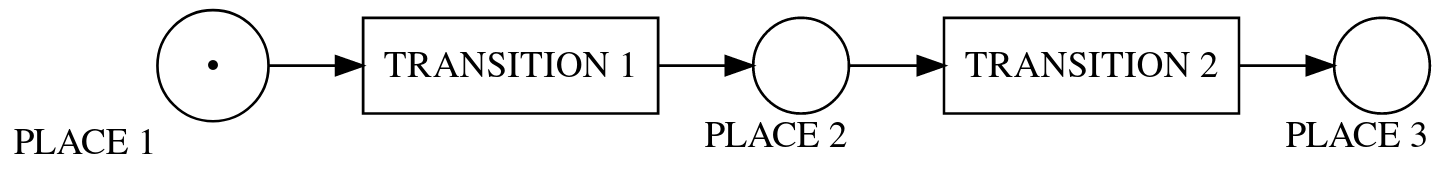
\includegraphics[scale=0.25]{petri-net-example.png}
    \caption{Example of a Petri net. \uppercase{PLACE 1} contains a token.}
    \label{fig:petri-net-example}
\end{figure}

When a transition fires, it consumes tokens from its input places and
produces tokens in its output places, reflecting a change in the state of the system.
The firing of a transition is enabled when there are sufficient tokens in its input places.
In Figure \ref{fig:petri-net-transition-firing-example}, we can see how successive firings happen.

\begin{figure}[H]
    \centering
    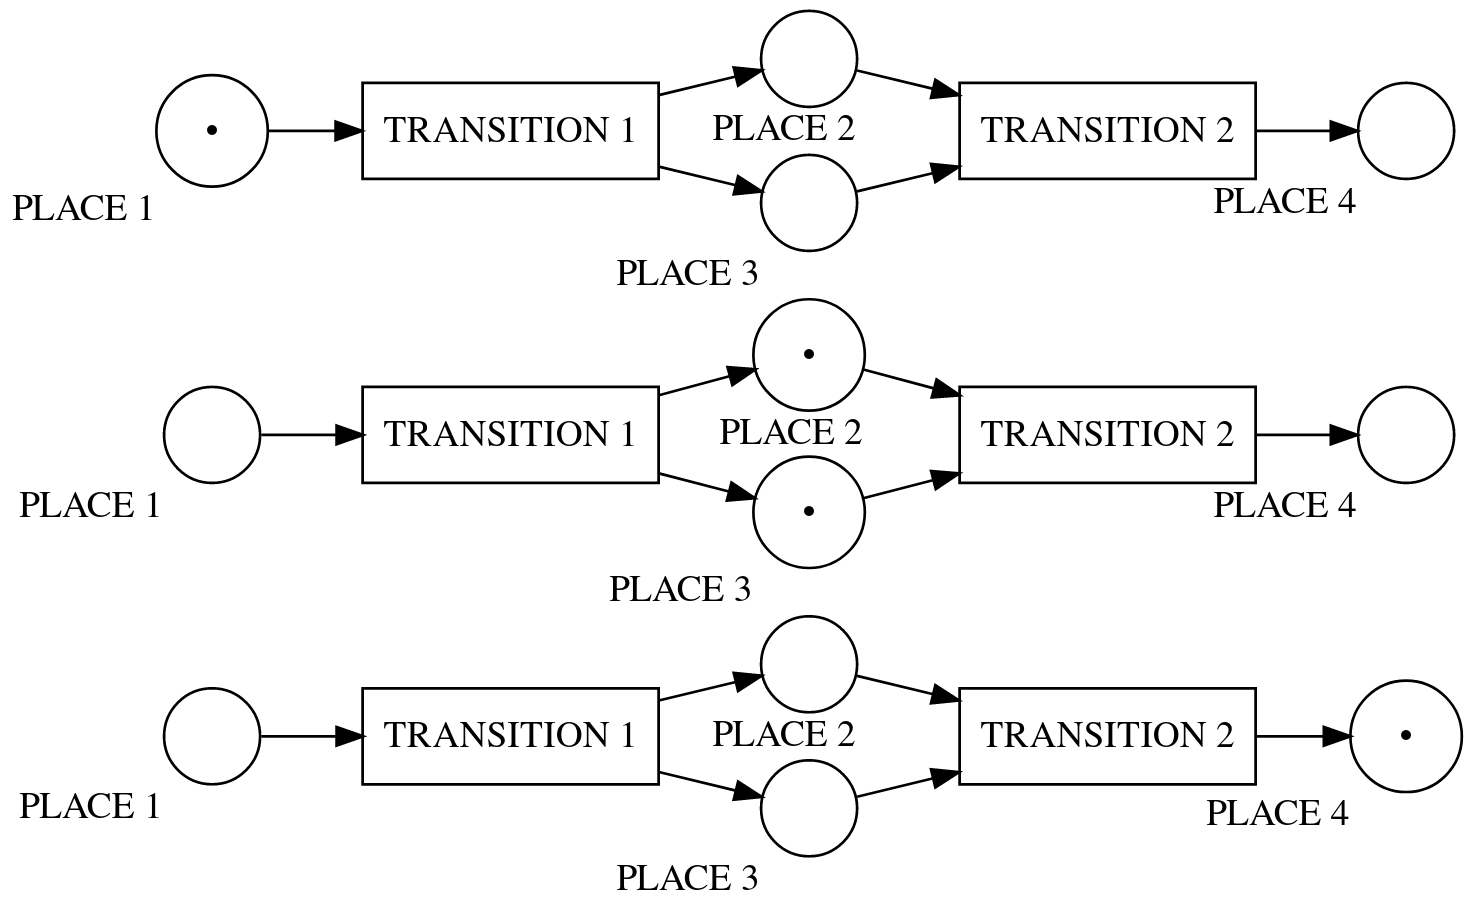
\includegraphics[scale=0.25]{petri-net-transition-firing-example.png}
    \caption{Example of transition firing: Transition 1 fires first, then transition 2 fires.}
    \label{fig:petri-net-transition-firing-example}
\end{figure}

The firing of enabled transitions is not deterministic, i.e., they fire randomly as long as they are enabled.
A disabled transition is considered \textbf{dead} if there is no reachable state in the system that can lead to the transition being enabled.
If all the transitions in the net are dead, then the net is considered \textbf{dead} too.
This state is analogous to the deadlock of a computer program.

Petri nets can be used to model and analyze a wide range of systems,
from simple systems with a few components to complex systems with many interacting components.
They can be used to detect potential problems in a system, optimize system performance and design and implement systems more effectively.

In particular, Petri nets can be used to detect deadlocks in source code by modeling the input program as a Petri net
and then analyzing the structure of the resulting net.
It will be shown that this approach is formally sound and
practicably amenable to source code written in the Rust programming language.

\subsection{Formal mathematical model}

A Petri net is a particular kind of bipartite, weighted, directed graph, equipped with an initial state called the \textit{initial marking}, $M_{0}$.
For this work, the following general definition of a Petri net taken from \cite{murata1989} will be used.

\begin{definition}[Petri net]
    A Petri net is a 5-tuple, $ PN = (P, T, F, W, M_{0}) $ where:

    \begin{quote}
        $ P = \{ p_1, p_2, \dots, p_m \} $ is a finite set of places,\\
        $ T = \{ t_1, t_2, \dots, t_n \} $ is a finite set of transitions,\\
        $ F \subseteq (P \times T) \cup (T \times P) $ is a set of arcs (flow relation),\\
        $ W: F \leftarrow \{1, 2, 3, ... \} $ is a weight function for the arcs,\\
        $ M_{0}: P \leftarrow \{0, 1, 2, 3, .... \} $ is the initial marking,\\
        $ P \cap T = \varnothing $ and $ P \cup T \neq \varnothing $
    \end{quote}
\end{definition}

In the graphical representation, arcs are labeled with their weight, which is a non-negative integer $k$.
Usually, the weight is omitted if it is equal to 1.
A $k$-weighted arc can be interpreted as a set of $k$ distinct parallel arcs.

A \textit{marking (state)} associates with each place a non-negative integer $l$.
If a marking assigns to place $p$ a non-negative integer $l$, we say that $p$ is \textit{marked with $l$ tokens}.
Pictorially, we denote his by placing $l$ black dots (tokens) in place $p$.
The \textit{pth} component of $M$, denoted by $M(p)$, is the number of tokens in place $p$.

An alternative definition of Petri nets uses \textit{bags} instead of a set to define the arcs, thus allowing multiple elements to be present.
It can be found in the literature, e.g., \cite[Definition 2.3]{peterson1981}.

As an example, consider the Petri net $ PN_{1} = (P, T, F, W, M) $ where:

\begin{quote}
    $ P = \{ p_1, p_2 \} $,\\
    $ T = \{ t_1, t_2 \} $,\\
    $ F = \{ (p_1, t_1), (p_2, t_2), (t_1, p_2), (t_2, p_2) \} $,\\
    $ W(a_i) = 1 \quad \forall a_i \in F $\\
    $ M(p_1) = 0, M(p_2) = 0 $
\end{quote}

This net contains no tokens and all the arc weights are equal to 1.
It is shown in Figure \ref{fig:petri-net-formal-example}.

\begin{figure}[H]
    \centering
    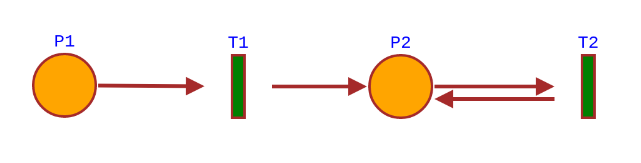
\includegraphics[scale=0.50]{petri-net-formal-example.png}
    \caption{Example of a small Petri net containing a self-loop}
    \label{fig:petri-net-formal-example}
\end{figure}

Figure \ref{fig:petri-net-formal-example} contains an interesting structure that we will encounter later.
This motivates the following definition.

\begin{definition}[Self-loop]
    A place node $p$ and a transition node $t$ define a self-loop if $p$ is both an input place and an output place of $t$.
\end{definition}

In most cases, we are interested in Petri nets containing no self-loops, which are called \textit{pure}.

\begin{definition}[Pure Petri net]
    A Petri net is said to be \textit{pure} if it has no self-loops.
\end{definition}

Moreover, if every arc weight is equal to one, we call the Petri net \textit{ordinary}.

\begin{definition}
    A Petri net is said to be \textit{ordinary} if all of its arc weights are 1's, i.e.
    \begin{equation*}
        W(a) = 1 \quad \forall a \in F
    \end{equation*}
\end{definition}

\subsection{Transition firing}

The transition firing rule is the core concept in Petri nets.
Despite being deceptively simple, its implications are far-reaching and complex.

\begin{definition}[Transition firing rule]
    Let $ PN = (P, T, F, W, M_{0}) $ be a Petri net.
    \begin{enumerate}[label=(\roman*)]
        \item A transition $t$ is said to be \textit{enabled} if each input place $p$ of $t$
              is marked with at least $W(p, t)$ tokens, where $W(p,t)$ is the weight of the arc from $p$ to $t$.
        \item An enabled transition may or may not fire (depending on whether or not the event takes place).
        \item A firing of an enabled transition $t$ removes $W(t,p)$ tokens from each input place $p$ of $t$,
              where $W(t, p)$ is the weight of the arc from $t$ to $p$.
    \end{enumerate}
\end{definition}

Transitions without input places or output places receive a special name.

\begin{definition}[Source transition]
    A transition without any input place is called a \textit{source transition}.
\end{definition}

\begin{definition}[Sink transition]
    A transition without any output place is called a \textit{sink transition}.
\end{definition}

It is important to note that a source transition is unconditionally enabled
and produces tokens without consuming any, while the firing of a sink transition
consumes tokens without producing any.

\subsection{Modeling examples}

In this subsection, several simple examples are presented to introduce
some basic concepts of Petri nets that are useful in modeling.
This subsection has been adapted from \cite{murata1989}.

\subsubsection{Finite-state machines}

Finite state machines can be represented by a subclass of Petri nets.

As an example of a finite-state machine, consider a coffee vending machine.
It accepts \EUR{1} or \EUR{2} coins and sells two types of coffee, the first costs \EUR{3} and the second \EUR{4}.
Assume that the machine can hold up to \EUR{4} and does not return any change.
Then, the state diagram of the machine can be represented by the Petri net shown in Figure \ref{fig:state-machine-example}.

\begin{figure}[H]
    \centering
    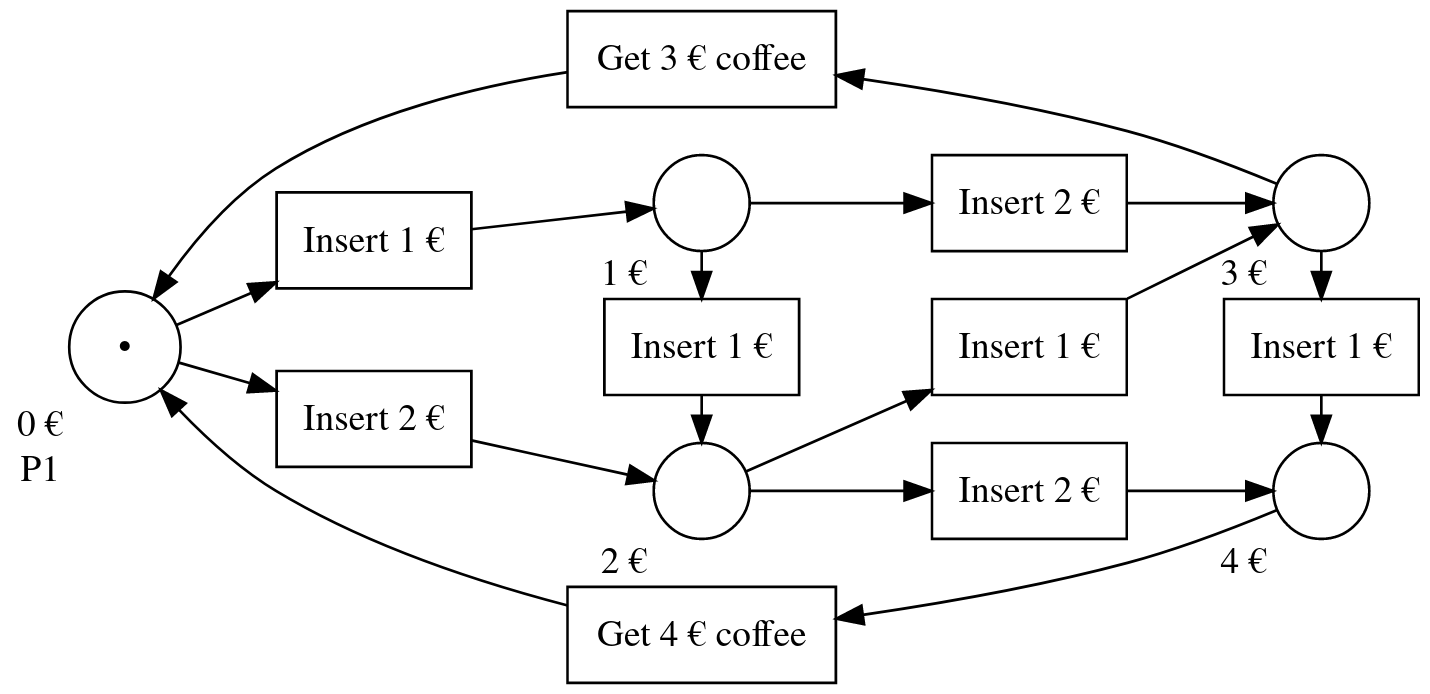
\includegraphics[scale=0.30]{state-machine-example.png}
    \caption{The Petri net for a coffee vending machine. It is equivalent to a state diagram.}
    \label{fig:state-machine-example}
\end{figure}

The transitions represent the insertion of a coin of the labeled value, e.g. ``Insert \EUR{1} coin''.
The places represent a possible state of the machine, i.e. the amount of money currently stored inside.
The place labeled \uppercase{P1} is marked with a token and corresponds to the initial state of the system.

We can now present the following definition of this subclass of Petri nets.

\begin{definition}[State machines]
    A Petri net in which each transition has exactly one incoming arc
    and exactly one outgoing arc is known as a \textit{state machine}.

    Any finite-state machine (or its state diagram) can be modeled with a state machine.
\end{definition}

The structure of a place $p_1$ having two (or more) output transitions $t_1$ and $t_2$ is called
a \textit{conflict}, \textit{decision} or \textit{choice}, depending on the application.
This is seen in the initial place \uppercase{P1} of Figure 1.4, where the user must select which coin to insert.

\subsubsection{Parallel activities}

Contrary to finite-state machines, Petri nets can model parallel or concurrent activities.

\section{The Rust programming language}

\section{Deadlocks}

\section{Lost signals}

\section{Compiler arquitecture}

\section{Model checking}

\bigskip